\documentclass{article}
\usepackage{tikz}
\usetikzlibrary{decorations.pathreplacing}

\begin{document}

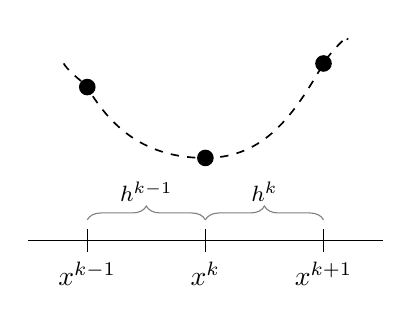
\begin{tikzpicture}[scale=1.5]

% x-axis
\draw[-] (-1.5,0) -- (1.5,0);
\draw (0, 0.1) -- (0, -0.1) node [below] {$x^k$};
\draw (-1, 0.1) -- (-1, -0.1) node [below] {$x^{k-1}$};
\draw (1, 0.1) -- (1, -0.1) node [below] {$x^{k+1}$};

% points
\fill (-1, 1.3) circle (2pt);
\fill (0, 0.7) circle (2pt);
\fill (1, 1.5) circle (2pt);

% line representing function
\draw [dashed, semithick]  
   (-1.2,1.5) to [out=-60,in=330] (-1,1.3)
   to [out=-60,in=180] (0,0.7) 
   to [out=0,in=240] (1,1.5)
   to [out=60,in=60] (1.2,1.7);

\draw [gray,decorate,decoration={brace,amplitude=5pt},yshift=5pt]
   (0,0)  -- (1,0) 
   node [black,midway,above=3pt] {\footnotesize $h^k$};
\draw [gray,decorate,decoration={brace,amplitude=5pt},yshift=5pt]
   (-1,0)  -- (0,0) 
   node [black,midway,above=3pt] {\footnotesize $h^{k-1}$};

\end{tikzpicture}

\end{document}
